\documentclass[crop, tikz, border=0pt]{standalone}
%\usetikzlibrary{...}% tikz package already loaded by 'tikz' option
\usetikzlibrary{matrix}
\usepackage{verbatim}
 \usetikzlibrary{decorations.text}
\definecolor{mygray}{RGB}{208,208,208}
\definecolor{myblue}{RGB}{226,0,116}
\usetikzlibrary{arrows}

\newcommand*{\mytextstyle}{\sffamily\Large\bfseries\color{mygray}}
\newcommand{\arcarrow}[3]{%
   % inner radius, middle radius, outer radius, start angle,
   % end angle, tip protusion angle, options, text
   \pgfmathsetmacro{\rin}{2}
   \pgfmathsetmacro{\rmid}{2.35}
   \pgfmathsetmacro{\rout}{2.7}
   \pgfmathsetmacro{\astart}{#1}
   \pgfmathsetmacro{\aend}{#2}
   \pgfmathsetmacro{\atip}{5}
   \fill[yellow, very thick] (\astart+\atip:\rin)
                         arc (\astart+\atip:\aend:\rin)
      -- (\aend-\atip:\rmid)
      -- (\aend:\rout)   arc (\aend:\astart+\atip:\rout)
      -- (\astart:\rmid) -- cycle;
   \path[
      decoration = {
         text along path,
         text = {|\mytextstyle|#3},
         text align = {align = center},
         raise = -1.0ex
      },
      decorate
   ](\astart+\atip:\rmid) arc (\astart+\atip:\aend+\atip:\rmid);
}
\usepackage{color}
\begin{document}
\color{yellow}
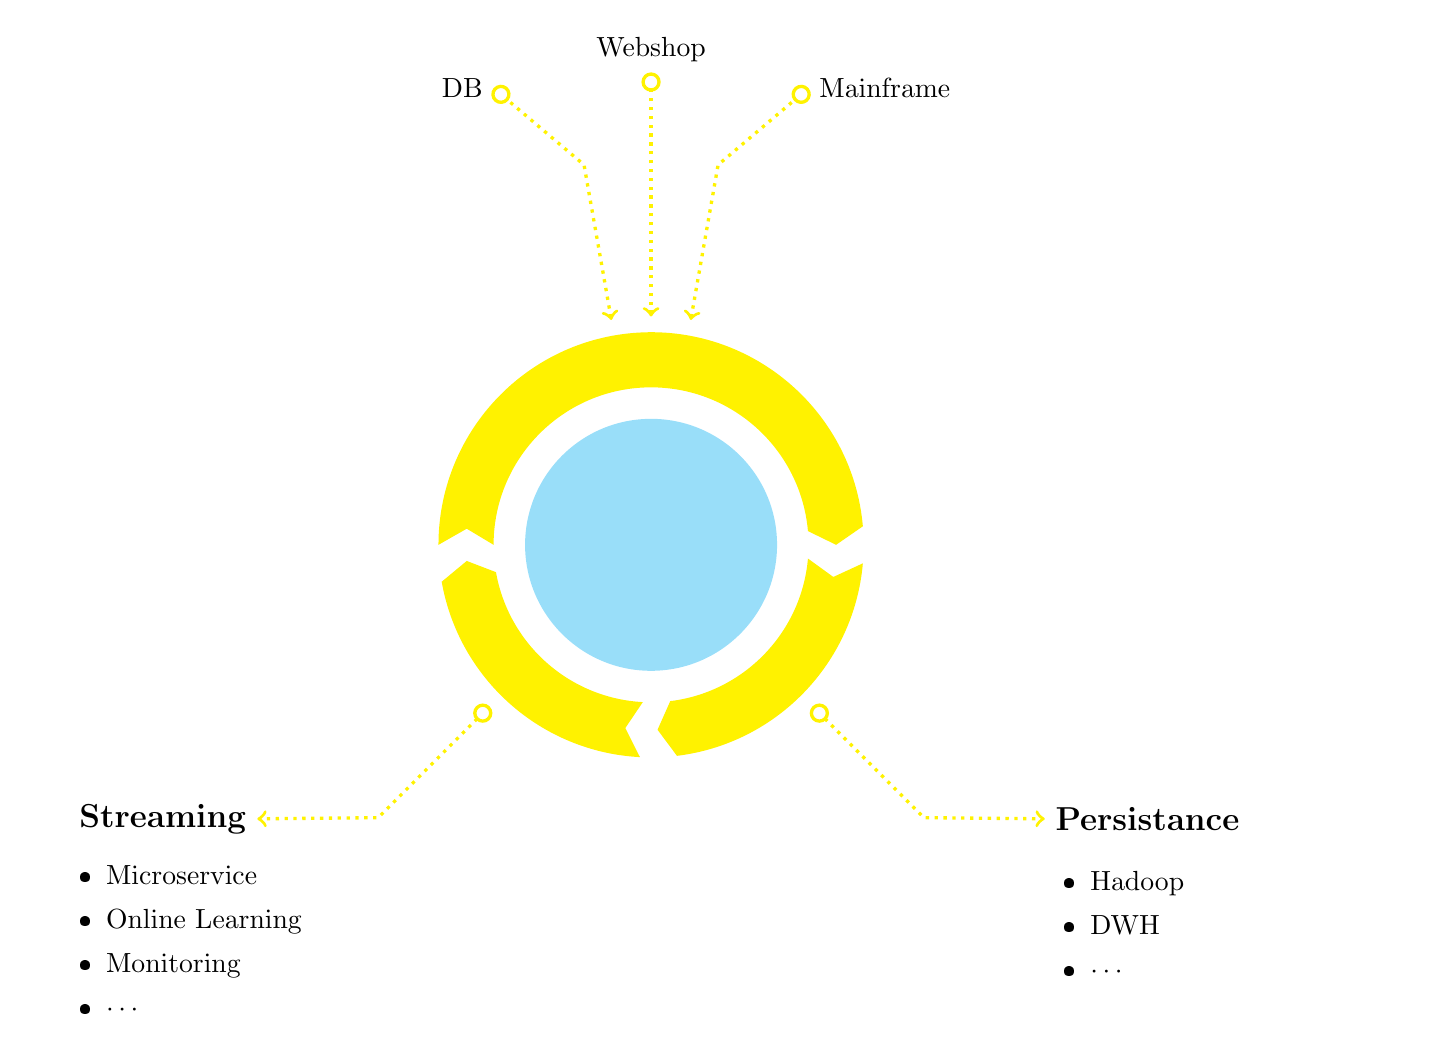
\begin{tikzpicture}[draw=yellow]

  
   \fill[even odd rule, cyan!40] circle (1.6);

%   \node at (0,0) [
%      font  = \mytextstyle,
%      color = mygray,
%      align = center
%   ]{
%      Data\\
%      lake
%   };
%   
   \arcarrow{175}{5}{}%{Input}
   \arcarrow{185}{267}{}%{Batch}
   \arcarrow{272}{355}{}%{Stream}
 
   
   \draw [dotted, very thick, <-o] (0,2.9) -- (0,6) node[above]{Webshop};
   \draw [dotted, very thick, <-o] (0.504, 2.856) -++ (80:2) --(2,5.8) node[right]{Mainframe};
\draw [dotted, very thick, <-o] (-0.504, 2.856) -++ (100:2) --(-2,5.8) node[left]{DB};

\draw [dotted, very thick, o->] (2.051, -2.051) -++ (315:2) -- (5,-3.48)node[right]{\large\textbf{Persistance}};
\node [text width=5cm] at (7.2, -4.6) {
    \begin{itemize}
    \itemsep0em
    \item Hadoop
	\item DWH
	\item $\cdots$
    \end{itemize}
};

\draw [dotted, very thick, o->] (-2.051, -2.051) -++ (225:2) --(-5,-3.48) node[left]{\large\textbf{Streaming}};
\node [text width=5cm] at (-5.3, -4.8) {
    \begin{itemize}
    \itemsep0em
    \item Microservice
	\item Online Learning	
	\item Monitoring
	\item $\cdots$
    \end{itemize}
};


\end{tikzpicture}

\end{document}

